
% to choose your degree
% please un-comment just one of the following
\documentclass[bsc,frontabs,twoside,singlespacing,parskip]{infthesis} 
\usepackage{graphicx}
%\usepackage{natbib}
\graphicspath{ {images/} }

%	BASIC CRITERIA
%	-	Understanding of the problem
%	-	Completion of the project.
%	-	Quality of the work
%	-	Quality of the report

%	ADDITIONAL CRITERIA
%	-	Knowledge of the literature
%	-	Critical evaluation of previous work
%	-	Critical evaluation of own work
%	-	Justification of the design decisions
%	-	Solution of any conceptual problems
%	-	Amount of work

%	EXCEPTIONAL CRITERIA
%	-	Evidence of originality
%	-	Outstanding scholarship and/or publishable research

\begin{document}

\title{Text Driven Talking Heads}

\author{Iain Brown}
\course{Computer Science}
\project{Undergraduate Dissertation} 
%\project{Undergraduate Thesis} % AI%Psy
%\project{4th Year Project Report}

\date{\today}
%\abstract{The aim of this project is to build a head motion synthesizer for a lifelike animated avatar. The head motions will be predicted entirely from the text of transcribed speech with the aim of finding a mapping between the text and natural head motions. Unlike previous areas of research where the head motions are generated from recorded speech.}
\maketitle
%\section*{Acknowledgements}
%Acknowledgements go here. 
\tableofcontents

% ============================================================= %
\chapter{Introduction}
- Head motion is very important when it comes to human communicatio\\
- Dialogue is much harder to fully understand without the non-verbal information\\
- Generating Lifelike avatars in many applications, VR, video games, shopping assistant \\
- Realistic head motions are vital otherwise humans may feel weird interacting with an avatar \\

% ============================================================= %
\chapter{Background Information}
\section{Data and Task}
\subsection{Recordings}
- Participants asked to read fairy tails \\
- Wearing Motion capture software \\
- Recordings transcribed \\
\subsection{Euler Angles}
- Commonly used in robotics \\
- Represent 3 dimensional movements in terms of 3 variables\\

\begin{center}
	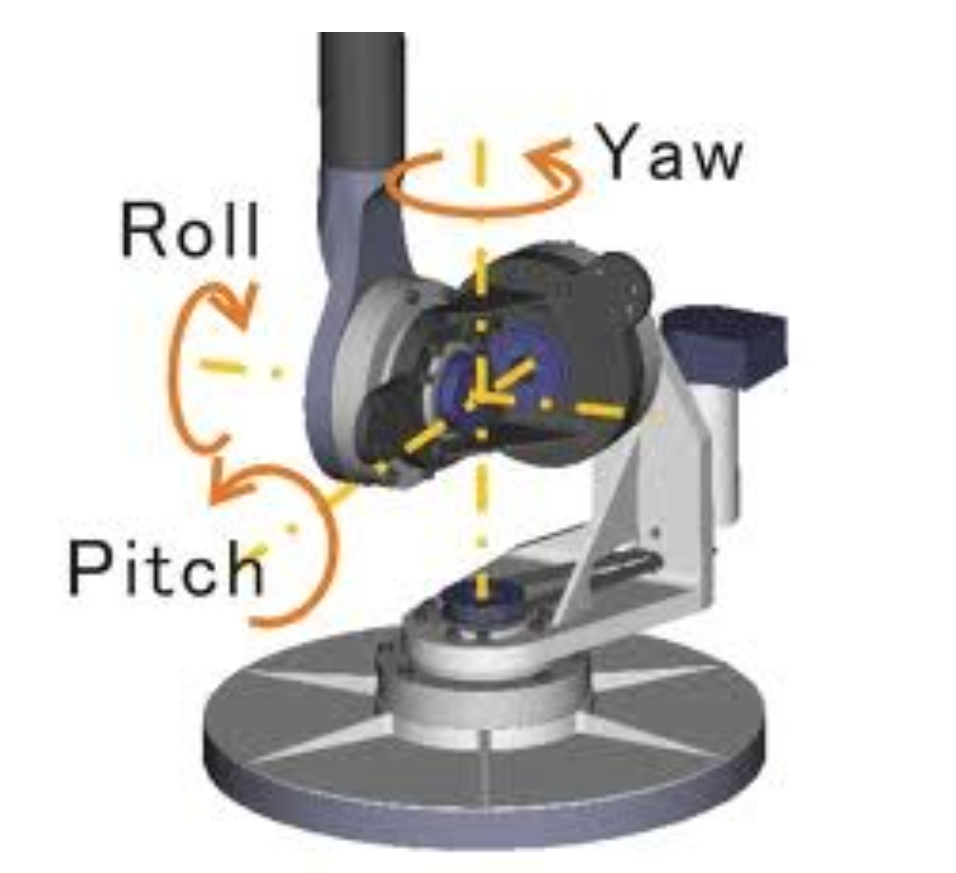
\includegraphics[width=.5\textwidth]{euler_angles.png}
\end{center}
\section{Hypotheses}
\subsection{Prosodic Features}
\subsection{Speech Content}
\subsection{Phrasing}
\subsection{Sentiment}
\section{Tools}
\subsection{Festival}
\subsection{Poser}
% ============================================================= %
\chapter{Text-Driven Head Motion Synthesis}
% This will be the theoretical implementation details 


% - To develop a system that is capable of synthesising a life-like talking head from text.
% - use a text to speech system to symnthesize the audio and save data about the audio
% - Build a mapping of words and sentences to discrete head motions
% - Make the system similar to real life (i.e recorded speech)
% - use Poser to animate the head motions
The goal of this project was to develop a system that was capable of synthesising life-like, realistic head motions from transcribed speech. The project aimed to 
\section{Text analysis}
\subsection{Festival}

\section{Head Motion Synthesis}

% ============================================================= %
\chapter{Implementation}

\section{Basic System}
\subsection{Trignomietric Functions}

\section{Random System}
\subsection{Discrete Head Motions}
\subsection{Comments}
\subsection{Bezier Smoothing}

\section{Rule-Based System}
\subsection{Parametric Smoothing}
	
% ============================================================= %
\chapter{Evaluation}

To evaluate the Text-Driven Head Motion System I performed both subjective analysis and objective analysis. The aim for the project was to develop a system which generates life-like talking heads with head motions that seem realistic and natural so it was important for humans to evaluate if the head motions were natural or not. Having a unit of measurement describing how close to the original head motions was also necessary in evaluating the system.

\section{Subjective Analysis}

\subsection{Outline}

\subsection{Preliminary Results and feedback}

\subsection{Results}

- Volunteers\\
- 5 Video Clips of animated talking heads \\
- 3 from the TDTH system\\
- 2 taken from actual recordings \\
- All mapped to the same face \\

- Volunteers will be asked to rate on a scale of 1-5 how natural the head motions seem \\
- Focus only on the head motions \\
- Not told which are synthesised\\
- Not told about real recordings \\
- So volunteer does not know which were which\\

- Important to keep as much the same as possible\\
- Only change head motions\\
- Apply Dynamic Time Warping\\ 

\section{Objective Analysis}

- Calculate difference in Euler angles\\
- Compare each system to two recordings due to lack of transcriptions\\

\section{Conclusion}
% ============================================================= %
\chapter{Conclusions}

\section{System Overview}

\section{Discussion}
	\subsection{Classification and Regression Trees}
	\subsection{Data Driven System}
\section{Future Work}
	\subsection{Expansion of techniques}
	
\bibliographystyle{plain}
\bibliography{diss}

\end{document}
